\subsection{E1--E3: the diagnostic measures what the theory describes}
\label{sec:res-e1}

Across \EoneConfigs{} configurations, \EoneTrials{} trials each and three readouts ---
\EoneMeasurements{} calibrated interfaces in total --- the floor was violated
\EoneViolations{} times. This is a correctness check on the implementation rather than
evidence for Theorem~\ref{thm:floor}, and we report it as such.

The attainment ratio of the tied readout falls from \EoneTiedRatioMax{} at the lowest feature
load to \EoneTiedRatioMin{} at the highest (Table~\ref{tab:e1}, Fig.~\ref{fig:overview}a): a
random code is close to Welch-optimal in the mean-square sense once $F/d$ is large, since
$\E\langle\phi_i,\phi_j\rangle^2=1/d$ while $W(F,d)\to1/d$ from below. At $d=\EoneTopD$,
$F=\EoneTopF$ the tied ratio is \EoneTopTiedRatio{} and the pseudoinverse ratio is
\EoneTopPinvRatio, the latter being the closer of the two at high load. In all
\EoneTightFrameConfigs{} configurations the harmonic tight frame attains the floor to within
\EoneTightFrameDev{} of exact equality, confirming Proposition~\ref{prop:tight} at machine
precision. The Gaussian control, by contrast, reaches ratios as large as
\EoneGaussianRatioMax: the bound holds for it too, but nothing forces an arbitrary readout to
be anywhere near the floor, and the diagnostic's attainment ratio is therefore informative
across seven orders of magnitude rather than a formality.

Fig.~\ref{fig:overview}b shows threshold recovery at $F=d^2$. The transition moves right with
$d$, from $s_{95}=\EtwoSixFourSNF$ at $d=64$ to $s_{95}=\EtwoTwoFiveSixSNF$ at $d=256$. At
$d=256$ and $s=s_{95}$, thresholding is exact in at least $95\%$ of trials while the calibrated
linear interface retains a per-coordinate RMS error of \EtwoTwoFiveSixLinRms, which is
\EtwoTwoFiveSixLinRmsOverRoot{} times the $d^{-1/2}$ scale and above its own theoretical floor
of \EtwoTwoFiveSixLinRmsFloor. That pair of numbers is the criterion-separation witness of
Problem~\ref{prob:main}, measured.

The threshold is a hyperparameter, and $\theta=1/2$ is not a privileged choice. At
$d=\EtwoThetaDmax$ the recovery threshold moves from $s_{95}=\EtwoThetaZeroPFourSNF$ at
$\theta=0.4$ to $s_{95}=\EtwoThetaZeroPFiveSNF$ at $\theta=0.5$ and
$s_{95}=\EtwoThetaZeroPSixSNF$ at $\theta=0.6$. Raising it helps here because, with unit-norm codes and Boolean
states, active scores concentrate near one while inactive scores concentrate near zero, so a
higher cut trades false positives for false negatives favourably in this regime; the individual
interference terms are of course signed. Two limits on how far this ablation goes: the three thresholds re-decode
the \emph{same} trials rather than independent replications, so they show the sensitivity of the
decision rule and not of the sampling; and at the smallest width the effect is not merely
numerical --- at $d=64$, $\theta=0.4$ no sparsity reaches the $95\%$ level at all, so no
certificate exists there.

E3 confirms the energy scale (Fig.~\ref{fig:overview}c). Over \EthreeConfigs{} configurations
the ratio $E/(s/d)$ lies in $[\EthreeRatioMin,\EthreeRatioMax]$ --- the $s/d$ reference scale is
essentially exact for random codes --- with \EthreeViolations{} violations of either energy
floor, and the closed forms agree with a \EthreeMcTrials-draw Monte Carlo estimate to within a
relative \EthreeMcMaxRelDiff.

Measured against the \emph{proved} uniform-support floor of
Proposition~\ref{prop:uniform-energy}, however, the ratio lies in
$[\EthreeUniformOverFloorMin,\EthreeUniformOverFloorMax]$: the bound is correct but conservative
by a factor between one and two in this regime. That is expected and worth stating plainly,
since it bounds what the diagnostic can certify. Two steps of the proof give the slack: the
non-negative $q\norm{A\mathbf 1}^2$ term is discarded, and $\norm{A}_F^2$ is replaced by its
worst case $F(F-d)/d$ rather than the value realised by the code at hand. The looser the
feature load, the larger the second effect --- here $F=8d$, so $(F-d)/F=7/8$ alone accounts for
part of the gap. Algorithm~\ref{alg:two} therefore reports the \emph{exact} energy computed
from the code's own frame operator, and uses the floor only as the guarantee that the quantity
can never be zero.

\begin{figure}[t]
\centering
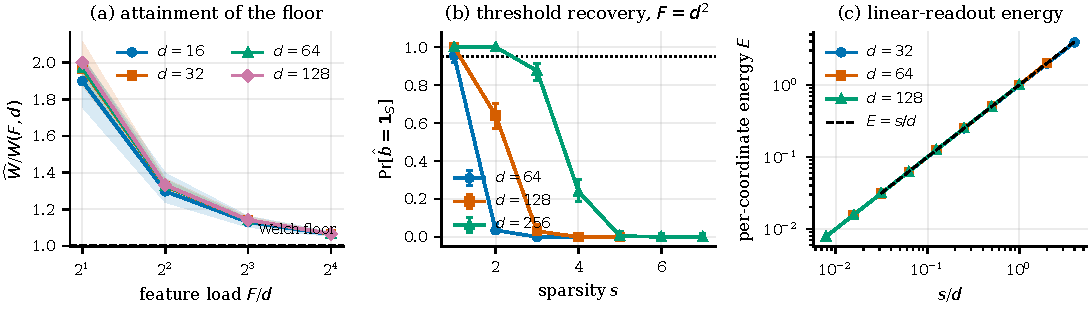
\includegraphics[width=\linewidth]{figures/fig1_diagnostic_overview.pdf}
\caption{\textbf{The Interface Diagnostic on random codes.} (a) Attainment ratio
$\widehat W/W(F,d)$ of the calibrated tied readout versus feature load; shaded bands are the
min--max range over trials, the dashed line is the floor of Theorem~\ref{thm:floor}.
(b) Exact threshold recovery at $F=d^2$ with Wilson $95\%$ intervals; the dotted line marks the
$0.95$ level defining $s_{95}$. (c) Average per-coordinate linear energy under uniformly random
supports against the $s/d$ reference. Generated by \code{scripts/make\_figures.py} from
\code{results/e1}, \code{results/e2} and \code{results/e3}.}
\label{fig:overview}
\end{figure}

\begin{table}[t]
\centering
\caption{E1: attainment ratio $\widehat W/W(F,d)$ of the calibrated tied readout for random
unit-norm codes, averaged over \EoneTrials{} trials. Values above one are required by
Theorem~\ref{thm:floor}; the approach to one with growing feature load is the content of the
measurement.}
\label{tab:e1}
\small
% Generated by scripts/make_tables.py from results/. Do not edit by hand.
\begin{tabular}{rrrrr}
\toprule
& \multicolumn{4}{c}{$F/d$} \\
\cmidrule(lr){2-5}
$d$ & 2 & 4 & 8 & 16 \\
\midrule
16 & 1.899 & 1.298 & 1.130 & 1.063 \\
32 & 1.966 & 1.327 & 1.141 & 1.065 \\
64 & 1.972 & 1.329 & 1.141 & 1.066 \\
128 & 1.999 & 1.332 & 1.141 & 1.066 \\
\bottomrule
\end{tabular}

\end{table}

